\section{}
A system is shown in the figure. Air (\(\rho = 0.97 \, \text{kg/m}^3\)) flows into surface 1 and flows out of surface 2. 
If \(v_1 = 5.6 \, \text{m/s}\), determine:


\begin{enumerate}[label=(\alph*)]
    \item the mass flow rate of air, and
    \item \(v_2\).
\end{enumerate}

\begin{figure}[h]
    \centering
    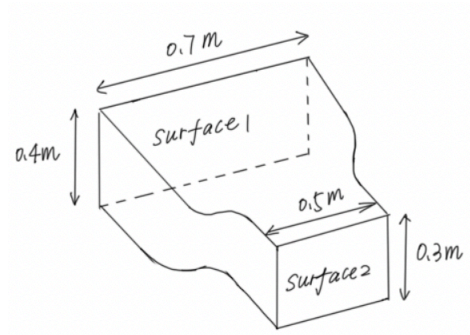
\includegraphics[width=0.3\textwidth]{Questions/Figures/Q2ProblemDiagram.png}
    \caption{Piston-cylinder device}
    \label{fig:Q2ProblemDiagram}
\end{figure}

\subsection{}
Assumptions
\begin{enumerate}
    \item Steady flow
    \item Incompressible flow
    \item Constant density
\end{enumerate}


The mass flow rate of air is given by:
\begin{align}
    \dot{m} &= \rho A_1 v_1 \nonumber \\
    &= (0.97)(0.4\times0.7)(5.6) \nonumber \\
    &= \boxed{\qty{1.521}{\kilogram\per\second}} \nonumber
\end{align}

\subsection{}
By conservation of mass, the mass flow rate at surface 2 is equal to the mass flow rate at surface 1, assuming steady flow. 

\begin{align*}
    v_2 = \frac{\dot{m}}{\rho A} &= \frac{1.521}{(0.97)(0.5\times0.3)} \\
    &= \boxed{\qty{10.454}{\meter\per\second}}
\end{align*}

